\documentclass[14pt]{extbook}
\usepackage{multicol, enumerate, enumitem, hyperref, color, soul, setspace, parskip, fancyhdr} %General Packages
\usepackage{amssymb, amsthm, amsmath, bbm, latexsym, units, mathtools} %Math Packages
\everymath{\displaystyle} %All math in Display Style
% Packages with additional options
\usepackage[headsep=0.5cm,headheight=12pt, left=1 in,right= 1 in,top= 1 in,bottom= 1 in]{geometry}
\usepackage[usenames,dvipsnames]{xcolor}
\usepackage{dashrule}  % Package to use the command below to create lines between items
\newcommand{\litem}[1]{\item#1\hspace*{-1cm}\rule{\textwidth}{0.4pt}}
\pagestyle{fancy}
\lhead{Progress Quiz 5}
\chead{}
\rhead{Version C}
\lfoot{9912-2038}
\cfoot{}
\rfoot{Spring 2021}
\begin{document}

\begin{enumerate}
\litem{
Factor the quadratic below. Then, choose the intervals that contain the constants in the form $(ax+b)(cx+d); b \leq d.$\[ 36x^{2} -60 x + 25 \]\begin{enumerate}[label=\Alph*.]
\item \( a \in [1.93, 2.67], \hspace*{5mm} b \in [-5, -2], \hspace*{5mm} c \in [15.5, 18.1], \text{ and } \hspace*{5mm} d \in [-5, 5] \)
\item \( a \in [4.29, 7.57], \hspace*{5mm} b \in [-5, -2], \hspace*{5mm} c \in [5, 7.2], \text{ and } \hspace*{5mm} d \in [-5, 5] \)
\item \( a \in [10.79, 13.74], \hspace*{5mm} b \in [-5, -2], \hspace*{5mm} c \in [2.5, 4.4], \text{ and } \hspace*{5mm} d \in [-5, 5] \)
\item \( a \in [-0.12, 1.1], \hspace*{5mm} b \in [-32, -27], \hspace*{5mm} c \in [0.2, 1.3], \text{ and } \hspace*{5mm} d \in [-38, -29] \)
\item \( \text{None of the above.} \)

\end{enumerate} }
\litem{
Factor the quadratic below. Then, choose the intervals that contain the constants in the form $(ax+b)(cx+d); b \leq d.$\[ 36x^{2} +60 x + 25 \]\begin{enumerate}[label=\Alph*.]
\item \( a \in [17.7, 19.2], \hspace*{5mm} b \in [4, 10], \hspace*{5mm} c \in [1.8, 3.4], \text{ and } \hspace*{5mm} d \in [4, 7] \)
\item \( a \in [-0.7, 1.1], \hspace*{5mm} b \in [27, 36], \hspace*{5mm} c \in [0.1, 1.3], \text{ and } \hspace*{5mm} d \in [29, 36] \)
\item \( a \in [4.9, 8.9], \hspace*{5mm} b \in [4, 10], \hspace*{5mm} c \in [3.8, 6.4], \text{ and } \hspace*{5mm} d \in [4, 7] \)
\item \( a \in [2.1, 3.4], \hspace*{5mm} b \in [4, 10], \hspace*{5mm} c \in [11.9, 14.7], \text{ and } \hspace*{5mm} d \in [4, 7] \)
\item \( \text{None of the above.} \)

\end{enumerate} }
\litem{
Write the equation of the graph presented below in the form $f(x)=ax^2+bx+c$, assuming  $a=1$ or $a=-1$. Then, choose the intervals that $a, b,$ and $c$ belong to.
\begin{center}
    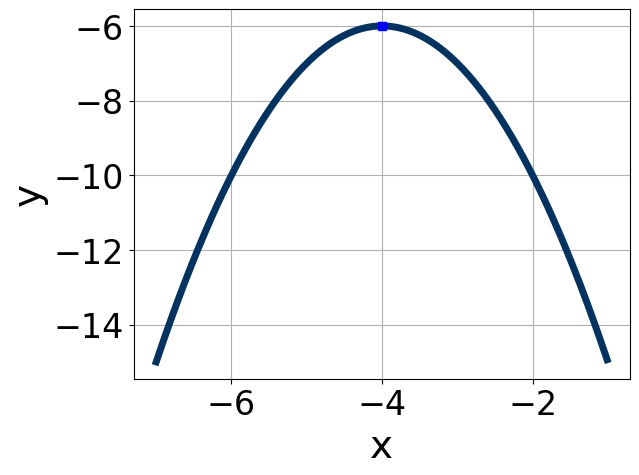
\includegraphics[width=0.5\textwidth]{../Figures/quadraticGraphToEquationC.png}
\end{center}
\begin{enumerate}[label=\Alph*.]
\item \( a \in [-1.5, 0.6], \hspace*{5mm} b \in [6, 11], \text{ and } \hspace*{5mm} c \in [-23, -20] \)
\item \( a \in [-1.5, 0.6], \hspace*{5mm} b \in [6, 11], \text{ and } \hspace*{5mm} c \in [-12, -7] \)
\item \( a \in [-1.5, 0.6], \hspace*{5mm} b \in [-8, -7], \text{ and } \hspace*{5mm} c \in [-23, -20] \)
\item \( a \in [0.4, 1.8], \hspace*{5mm} b \in [-8, -7], \text{ and } \hspace*{5mm} c \in [7, 13] \)
\item \( a \in [0.4, 1.8], \hspace*{5mm} b \in [6, 11], \text{ and } \hspace*{5mm} c \in [7, 13] \)

\end{enumerate} }
\litem{
Graph the equation below.\[ f(x) = (x-4)^2 + 19 \]\begin{enumerate}[label=\Alph*.]
\begin{multicols}{2}\item 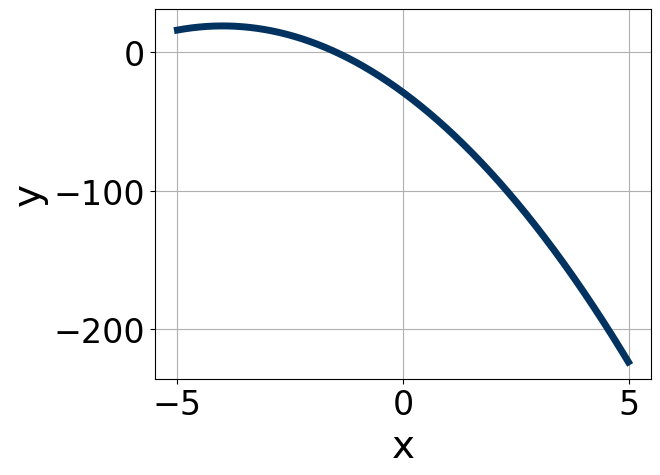
\includegraphics[width = 0.3\textwidth]{../Figures/quadraticEquationToGraphAC.png}\item 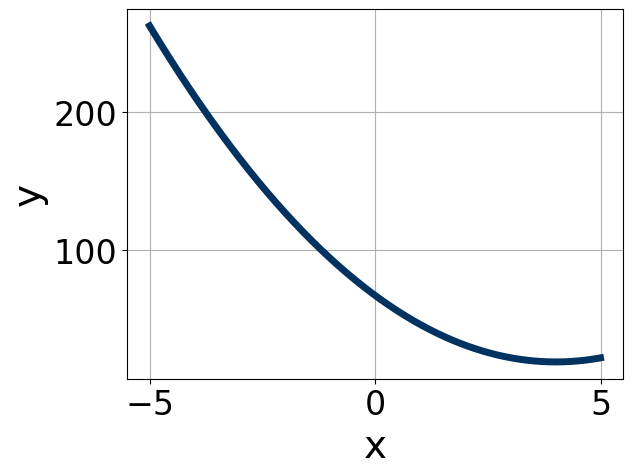
\includegraphics[width = 0.3\textwidth]{../Figures/quadraticEquationToGraphBC.png}\item 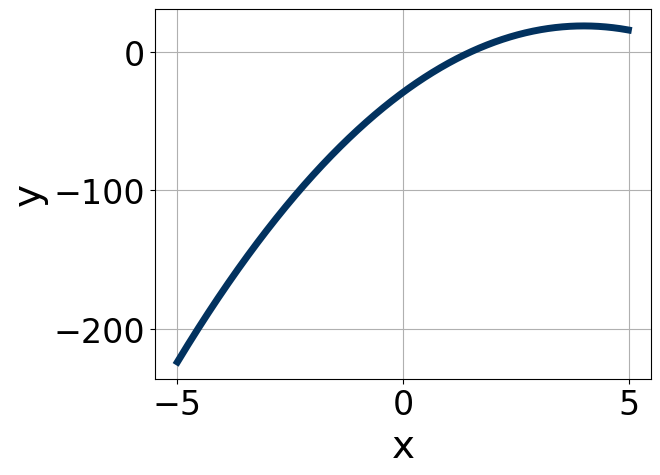
\includegraphics[width = 0.3\textwidth]{../Figures/quadraticEquationToGraphCC.png}\item 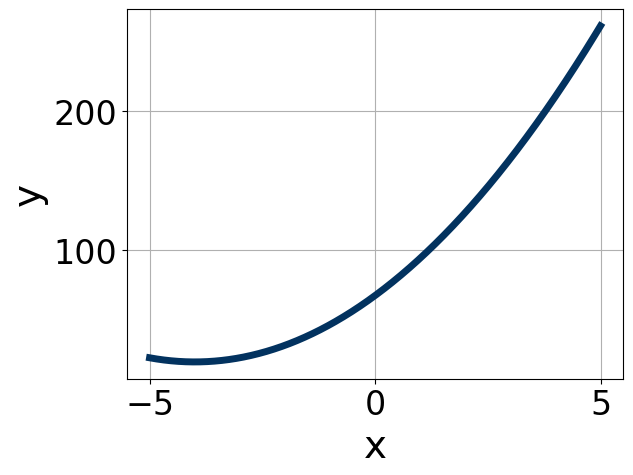
\includegraphics[width = 0.3\textwidth]{../Figures/quadraticEquationToGraphDC.png}\end{multicols}\item None of the above.
\end{enumerate} }
\litem{
Solve the quadratic equation below. Then, choose the intervals that the solutions $x_1$ and $x_2$ belong to, with $x_1 \leq x_2$.\[ 20x^{2} -21 x -54 = 0 \]\begin{enumerate}[label=\Alph*.]
\item \( x_1 \in [-1.74, -1.15] \text{ and } x_2 \in [1.8, 2.84] \)
\item \( x_1 \in [-3.76, -3.56] \text{ and } x_2 \in [0.5, 1.12] \)
\item \( x_1 \in [-0.82, -0.06] \text{ and } x_2 \in [6.28, 6.98] \)
\item \( x_1 \in [-24.37, -23.32] \text{ and } x_2 \in [44.99, 46.25] \)
\item \( x_1 \in [-6.23, -5.24] \text{ and } x_2 \in [-0.8, 0.56] \)

\end{enumerate} }
\litem{
Solve the quadratic equation below. Then, choose the intervals that the solutions belong to, with $x_1 \leq x_2$ (if they exist).\[ 14x^{2} +8 x -8 = 0 \]\begin{enumerate}[label=\Alph*.]
\item \( x_1 \in [-15.94, -15.23] \text{ and } x_2 \in [6.2, 7.49] \)
\item \( x_1 \in [-0.77, 0.05] \text{ and } x_2 \in [0.94, 1.12] \)
\item \( x_1 \in [-1.4, -0.63] \text{ and } x_2 \in [0.5, 0.79] \)
\item \( x_1 \in [-23.25, -21.33] \text{ and } x_2 \in [21.3, 22.48] \)
\item \( \text{There are no Real solutions.} \)

\end{enumerate} }
\litem{
Solve the quadratic equation below. Then, choose the intervals that the solutions $x_1$ and $x_2$ belong to, with $x_1 \leq x_2$.\[ 8x^{2} -54 x + 81 = 0 \]\begin{enumerate}[label=\Alph*.]
\item \( x_1 \in [0.62, 0.89] \text{ and } x_2 \in [13.16, 13.92] \)
\item \( x_1 \in [17.94, 18.23] \text{ and } x_2 \in [35.81, 36.56] \)
\item \( x_1 \in [0.97, 1.45] \text{ and } x_2 \in [8.37, 10.86] \)
\item \( x_1 \in [2.22, 2.27] \text{ and } x_2 \in [4.19, 4.84] \)
\item \( x_1 \in [1.44, 1.53] \text{ and } x_2 \in [5.44, 6.79] \)

\end{enumerate} }
\litem{
Write the equation of the graph presented below in the form $f(x)=ax^2+bx+c$, assuming  $a=1$ or $a=-1$. Then, choose the intervals that $a, b,$ and $c$ belong to.
\begin{center}
    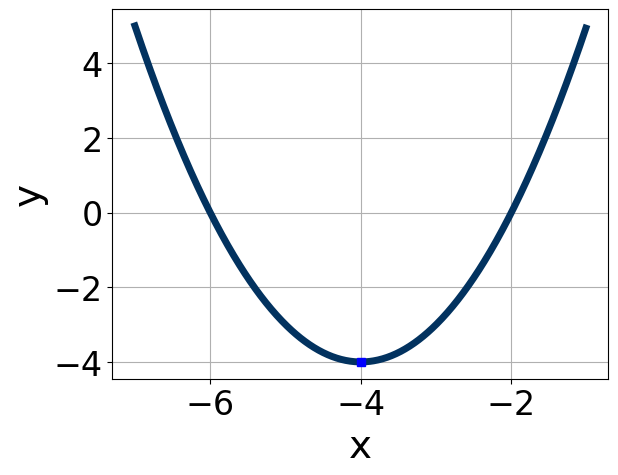
\includegraphics[width=0.5\textwidth]{../Figures/quadraticGraphToEquationCopyC.png}
\end{center}
\begin{enumerate}[label=\Alph*.]
\item \( a \in [-2.5, -0.7], \hspace*{5mm} b \in [5, 12], \text{ and } \hspace*{5mm} c \in [-20, -17] \)
\item \( a \in [-2.5, -0.7], \hspace*{5mm} b \in [-8, -6], \text{ and } \hspace*{5mm} c \in [-20, -17] \)
\item \( a \in [0.9, 1.2], \hspace*{5mm} b \in [-8, -6], \text{ and } \hspace*{5mm} c \in [18, 22] \)
\item \( a \in [0.9, 1.2], \hspace*{5mm} b \in [5, 12], \text{ and } \hspace*{5mm} c \in [11, 16] \)
\item \( a \in [0.9, 1.2], \hspace*{5mm} b \in [-8, -6], \text{ and } \hspace*{5mm} c \in [11, 16] \)

\end{enumerate} }
\litem{
Solve the quadratic equation below. Then, choose the intervals that the solutions belong to, with $x_1 \leq x_2$ (if they exist).\[ 19x^{2} +8 x -9 = 0 \]\begin{enumerate}[label=\Alph*.]
\item \( x_1 \in [-0.76, -0.23] \text{ and } x_2 \in [0.92, 0.94] \)
\item \( x_1 \in [-28.07, -26.93] \text{ and } x_2 \in [27.07, 27.42] \)
\item \( x_1 \in [-17.94, -17.47] \text{ and } x_2 \in [9.4, 9.9] \)
\item \( x_1 \in [-1.2, -0.81] \text{ and } x_2 \in [0.08, 0.87] \)
\item \( \text{There are no Real solutions.} \)

\end{enumerate} }
\litem{
Graph the equation below.\[ f(x) = (x-1)^2 - 12 \]\begin{enumerate}[label=\Alph*.]
\begin{multicols}{2}\item 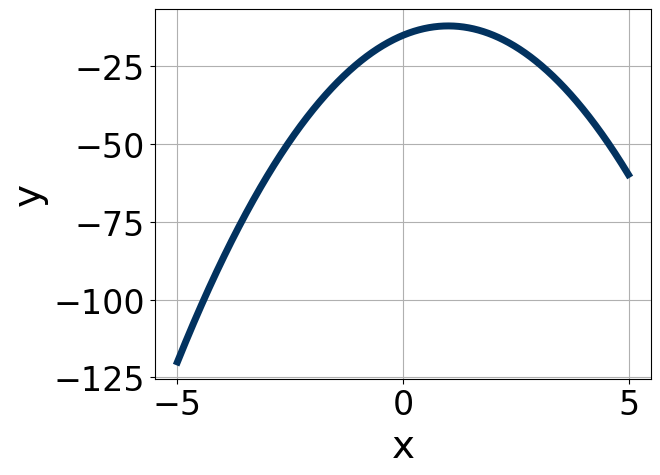
\includegraphics[width = 0.3\textwidth]{../Figures/quadraticEquationToGraphCopyAC.png}\item 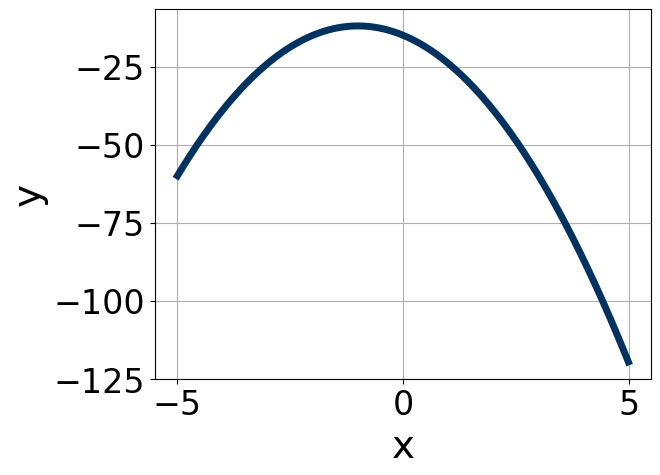
\includegraphics[width = 0.3\textwidth]{../Figures/quadraticEquationToGraphCopyBC.png}\item 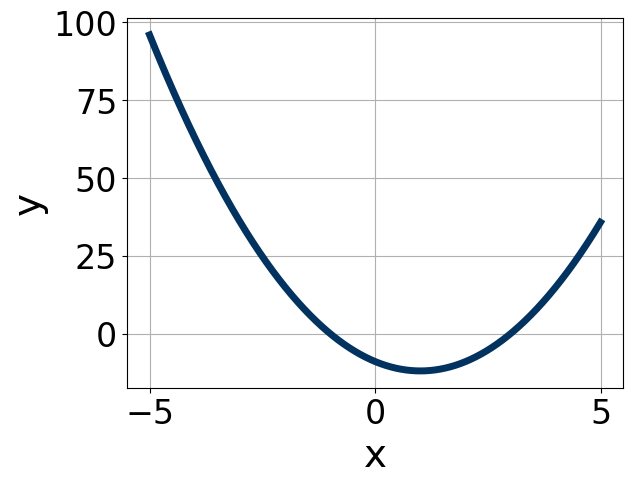
\includegraphics[width = 0.3\textwidth]{../Figures/quadraticEquationToGraphCopyCC.png}\item 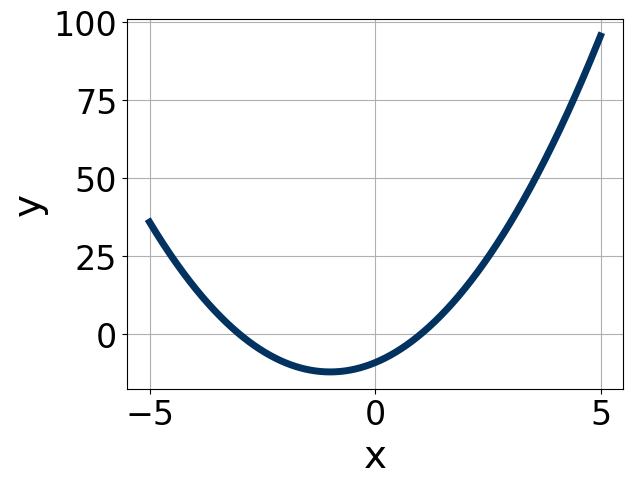
\includegraphics[width = 0.3\textwidth]{../Figures/quadraticEquationToGraphCopyDC.png}\end{multicols}\item None of the above.
\end{enumerate} }
\end{enumerate}

\end{document}